\documentclass[12pt]{article}
\usepackage[a4paper, margin=0.75in]{geometry}
\usepackage[document]{ragged2e}
\usepackage{graphicx}
\graphicspath{ {./images/} }
\usepackage{enumerate}
\usepackage{framed}
\usepackage{amsmath,amsfonts,amsthm,thmtools,amssymb,mathtools,commath}
\usepackage{physics}
\usepackage{tikz}
\usetikzlibrary{mindmap}
\usepackage{caption}
\usepackage{xcolor}
\usepackage[most]{tcolorbox}
\usepackage{cleveref}


%%%%%%%%%%%%%%%%
%  Definition  %
%%%%%%%%%%%%%%%%
\tcbuselibrary{theorems,skins,hooks}
\newtcbtheorem[number within=subsection]{definition}{Definition}%
{
    % theorem style=definition,
    enhanced,
	before skip=2mm,after skip=2mm, colback=cyan!5,colframe=cyan!80!black,boxrule=0.5mm,
	attach boxed title to top left={xshift=1cm,yshift*=1mm-\tcboxedtitleheight},
	boxed title style={frame code={
					\path[fill=cyan]
					([yshift=-1mm,xshift=-1mm]frame.north west)
					arc[start angle=0,end angle=180,radius=1mm]
					([yshift=-1mm,xshift=1mm]frame.north east)
					arc[start angle=180,end angle=0,radius=1mm];
					\path[left color=cyan!30!black,right color=cyan!30!black,
						middle color=cyan!50!black]
					([xshift=-2mm]frame.north west) -- ([xshift=2mm]frame.north east)
					[rounded corners=1mm]-- ([xshift=1mm,yshift=-1mm]frame.north east)
					-- (frame.south east) -- (frame.south west)
					-- ([xshift=-1mm,yshift=-1mm]frame.north west)
					[sharp corners]-- cycle;
				},interior engine=empty,
		},
	fonttitle=\bfseries,
	title={#2},#1
}{def}


%%%%%%%%%%%%%
%  Theorem  %
%%%%%%%%%%%%%
\tcbuselibrary{theorems,skins,hooks}
\newtcbtheorem[use counter from=definition]{theorem}{Theorem}%
{
    theorem style=plain,
    enhanced,
    colframe=green,
    boxrule=1pt,
    titlerule=0mm,
    toptitle=1mm,
    bottomtitle=1mm,
    fonttitle=\bfseries,
    fontupper=\mdseries\itshape,
    coltitle=green!30!black,
    colbacktitle=cyan!15!white,
    colback=green!10,
    description font=\bfseries\sffamily
}{thrm}


%%%%%%%%%%%%%%
% Corollary  %
%%%%%%%%%%%%%%
 \tcbuselibrary{theorems,skins}
 \newtcbtheorem[use counter from=theorem]{corollary}{Corollary}%
 {
    theorem style=plain,
    enhanced,
    colframe=green,
    frame hidden,
    titlerule=0mm,
    toptitle=1mm,
    bottomtitle=1mm,
    fonttitle=\bfseries,
    fontupper=\mdseries\itshape,
    coltitle=green!30!black,
    colbacktitle=cyan!15!white,
    colback=green!10,
    description font=\bfseries\sffamily
 }{corl}


%%%%%%%%%%%%%
%  Example  %
%%%%%%%%%%%%%
\tcbuselibrary{theorems,skins,hooks}
\newtcbtheorem[number within=section]{example}{Example}%
{
	enhanced,
	breakable,
	colback = gray!5,
	frame hidden,
	boxrule = 0sp,
	borderline west = {2pt}{0pt}{gray},
	sharp corners,
	detach title,
	before upper = \tcbtitle\par\smallskip,
    coltitle=gray!70!black,
	fonttitle = \bfseries\sffamily,
	description font = \mdseries\bfseries
}
{xmp}


%%%%%%%%%%%%%%
%  Exercise  %
%%%%%%%%%%%%%%
\tcbuselibrary{theorems,skins,hooks}
\newtcbtheorem[number within=section]{exercise}{Exercise}%
{
    enhanced,
    breakable,
    colback=black!5,
    colframe=black!30,
    left=0.5em,
    before skip=10pt,
    after skip=10pt,
    boxrule=0pt,
    boxsep=0pt,
    arc=0pt,
    outer arc=0pt,
    borderline west={3pt}{0pt}{black!30},
}{exc}

%%%%%%%%%%
%  Note  %
%%%%%%%%%%
\usetikzlibrary{arrows,calc,shadows.blur}
\tcbuselibrary{skins}
\newtcolorbox{note}[1][]{%
	enhanced jigsaw,
	colback=gray!20!white,%
	colframe=gray!80!black,
	size=small,
	boxrule=1pt,
	title=\textbf{Note:-},
	halign title=flush center,
	coltitle=black,
	breakable,
	drop shadow=black!50!white,
	attach boxed title to top left={xshift=1cm,yshift=-\tcboxedtitleheight/2,yshifttext=-\tcboxedtitleheight/2},
	minipage boxed title=1.5cm,
	boxed title style={%
			colback=white,
			size=fbox,
			boxrule=1pt,
			boxsep=2pt,
			underlay={%
					\coordinate (dotA) at ($(interior.west) + (-0.5pt,0)$);
					\coordinate (dotB) at ($(interior.east) + (0.5pt,0)$);
					\begin{scope}
						\clip (interior.north west) rectangle ([xshift=3ex]interior.east);
						\filldraw [white, blur shadow={shadow opacity=60, shadow yshift=-.75ex}, rounded corners=2pt] (interior.north west) rectangle (interior.south east);
					\end{scope}
					\begin{scope}[gray!80!black]
						\fill (dotA) circle (2pt);
						\fill (dotB) circle (2pt);
					\end{scope}
				},
		},
	#1,
}

\usepackage{makecell}
\allowdisplaybreaks

\title{
    \textbf{Simple Harmonic Motion}
}

\author{
    Turja Roy\\
    ID: 2108052
}
\date{}

\begin{document}
\maketitle
\tableofcontents
\newpage

\section{Oscillation and Vibration}
\subsection{Oscillation}
\begin{itemize}
    \item Oscillation is the repetitive variation, typically in time, of some measure about a central value (often a point of equilibrium) or between two or more different states.
    \item The term vibration is precisely used to describe mechanical oscillation.
    \item Familiar examples of oscillation include a swinging pendulum and alternating current.
\end{itemize}

\subsection{Vibration}
\begin{itemize}
    \item Vibration is a mechanical phenomenon whereby oscillations occur about an equilibrium point.
    \item The word comes from Latin vibrationem ("shaking, brandishing").
    \item The oscillations may be periodic, such as the motion of a pendulum—or random, such as the movement of a tire on a gravel road.
\end{itemize}

\subsection{Differences between Oscillation and Vibration}
\begin{itemize}
    \item Oscillation is the definite displacement of a body in terms of distance or time, whereas vibration is the movement brought about in a body due to oscillation.
    \item Oscillation takes place in physical, biological systems, and often in our society, but vibrations is associated with mechanical systems only.
    \item Oscillation is about a single body, whereas vibration is the result of collective oscillation of atoms in the body.
    \item All vibrations are oscillations, but not all oscillations are vibrations.
\end{itemize}

\section{Simple Harmonic Motion}
\subsection{Definition}

\begin{definition}{Simple Harmonic Motion}{}
    Simple harmonic motion is a type of periodic motion where the restoring force is directly proportional to the displacement and acts in the direction opposite to that of displacement.
\end{definition}

A particle is said to execute SHM when it will
\begin{enumerate}[(a)]
    \item Trace and retrace the same path over and over again.
    \item Change direction at a regular interval of time.
    \item Move along a straight line.
    \item Have acceleration proportional to its displacement from the mean position.
\end{enumerate}

A particle which satisfies the condition (a) only is said to execute \textbf{periodic motion}. A particle which satisfies condition (a) and (b) is said to execute \textbf{vibratory motion}. \\~\\

Let $P$ be a particle moving on the circumference of a circle of radius $r$ with a uniform velocity $v$. Let angular velocity be $\omega = v/r$.

\begin{figure}[htpb]
    \centering
    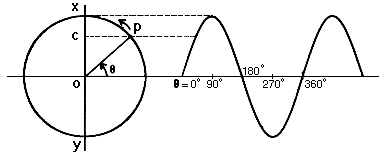
\includegraphics[width=0.5\textwidth]{1.png}
\end{figure}

\vspace{20pt}
Displacement of the particle from the mean position is given by $\displaystyle y = r \sin{\omega t}$\\
So, velocity of the particle is given by $\displaystyle v = \frac{dy}{dt} = \omega r \cos{\omega t}$\\
And acceleration of the particle is given by $\displaystyle a = \frac{dv}{dt} = -\omega^2 r \sin{\omega t} = -\omega^2 y$

\vspace{20pt}
\begin{center}
    \begin{tabular}{c | c | c | c | c}
        Angle & \makecell{Position of \\ vibrating particle} & \makecell{Displacement \\ $y = r \sin{\omega t}$} & \makecell{Velocity \\ $\displaystyle \dv{y}{t} = \omega r \cos{\omega t}$} & \makecell{Acceleration \\ $-\omega^2 r \sin{\omega t} = -\omega^2 y$} \\\hline\hline
        0 & O & 0 & $\omega r$ & 0 \\\hline
        $\pi/2$ & X & $r$ & 0 & $-\omega^2 a$ \\\hline
        $\pi$ & O & 0 & $-\omega r$ & 0 \\\hline
        $3\pi/2$ & Y & $-r$ & 0 & $\omega^2 r$ \\\hline
        $2\pi$ & O & 0 & $\omega r$ & 0
    \end{tabular}
\end{center}

\subsection{Differential Equation of SHM}
Let $y$ be the displacement of the particle from the mean position at time $t$, $r$ be the amplitude, and $\alpha$ be the epoch of the vibrating particle \\
\begin{equation}
    y = r \sin{(\omega t + \alpha)}
\end{equation}
\begin{equation}
    \dv{y}{t} = r \omega \cos{(\omega t + \alpha)}
\end{equation}
\begin{equation}
    \dv[2]{y}{t} = -r \omega^2 \sin{(\omega t + \alpha)}
\end{equation}

Hence the differential equation of SHM is
\begin{equation}
    \dv[2]{y}{t} + \omega^2 y = 0
\end{equation}

\subsection{Solution of the Differential Equation of SHM}
\begin{equation}
    \dv[2]{y}{t} + \omega^2 y = 0
\end{equation}

Here, \[
    \dv[2]{y}{t} = \dv{v}{t} = \dv{v}{y} \dv{y}{t} = v \dv{v}{y}
\]
\begin{align*}
    v \: d{v} + \omega^2y \: d{y} &= 0 \\
    \int{v} \: d{v} + \omega^2 \int{y} \: d{y} &= 0 \\
    \frac{v^2}{2} + \frac{\omega^2 y^2}{2} &= C' \\
    \left( \dv{y}{t} \right) ^2 + \omega^2 y^2 &= C^2
\end{align*}

At maximum displacement, $y = r$ and $\displaystyle \dv{y}{t} = 0$ \\
So, $C^2 = \omega^2 r^2$ \\
\begin{align*}
    \left( \dv{y}{t} \right)^2 &= \omega^2(r^2 - y^2) \\
    \dv{y}{t} &= \omega \sqrt{r^2 - y^2} \\
    \int{\frac{1}{\sqrt{r^2-y^2}}} \: d{y} &= \int{\omega} \: d{t} \\
    \sin^{-1}{\frac{y}{r}} &= \omega t + \alpha
\end{align*}
\begin{equation}
    \boxed{ y = r \sin{(\omega t + \alpha)} }
\end{equation}

By expanding equation (6), we get
\begin{equation}
    y = r \sin{\omega t} \cos{\alpha} + r \cos{\omega t} \sin{\alpha}
\end{equation}
If $y = 0$ at $t = 0$, then $\alpha = 0$ \\
\begin{equation}
    y = r \sin{\omega t}
\end{equation}
If $y = r$ at $t = 0$, then $\alpha = \pi/2$ \\
\begin{equation}
    y = r \cos{\omega t}
\end{equation}

Hence, the general solution of the differential equation of SHM is
\begin{equation}
    \boxed{ y = A \sin{\omega t} + B \cos{\omega t} }
\end{equation}

\section{Energy in SHM}
\subsection{Total Energy of a Vibrating Particle}
\begin{align*}
    \text{Kinetic Energy} &= \frac{1}{2} m \left( \dv{y}{t} \right)^2 \\
    &= \frac{1}{2} m \omega^2 r^2 \cos^2{(\omega t + \alpha)} \\
    \text{Potential Energy} &= \frac{1}{2} k y^2 \\
    &= \frac{1}{2} m \omega^2 r^2 \\
    &= \frac{1}{2} m \omega^2 r^2 \sin^2{(\omega t + \alpha)}
\end{align*}

Thus, the total energy of the vibrating particle is
\begin{equation}
    \boxed{ E = \frac{1}{2} k r^2 = \frac{1}{2} m \omega^2 r^2 }
\end{equation}

\begin{figure}[htpb]
    \centering
    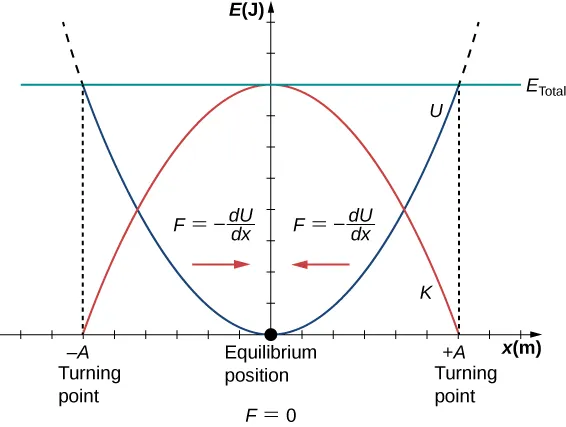
\includegraphics[width=0.5\textwidth]{2.png}
\end{figure}

\subsection{Average Kinetic Energy}
Kinetic energy of the particle is given by
\begin{equation}
    K = \frac{1}{2} m \left( \dv{y}{t} \right)^2 = \frac{1}{2} m \omega^2 r^2 \cos^2{(\omega t + \alpha)}
\end{equation}
Hence, average kinetic energy is
\begin{align*}
    \overline{K} &= \frac{1}{T} \int_{0}^{T} K \: dt \\
    &= \frac{1}{T} \int_{0}^{T} \frac{1}{2} m \omega^2 r^2 \cos^2{(\omega t + \alpha)} \: dt \\
    &= \frac{1}{2} m \omega^2 r^2 \frac{1}{T} \int_{0}^{T} \cos^2{(\omega t + \alpha)} \: dt \\
    &= \frac{1}{2} m \omega^2 r^2 \frac{1}{T} \int_{0}^{T} \frac{1 + \cos{2(\omega t + \alpha)}}{2} \: dt \\
    &= \frac{1}{2} m \omega^2 r^2 \frac{1}{T} \left[ \frac{t}{2} + \frac{\sin{2(\omega t + \alpha)}}{4\omega} \right]_{0}^{T} \\
    &= \frac{1}{2} m \omega^2 r^2 \frac{1}{T} \left[ \frac{T}{2} + \frac{\sin{2(\omega T + \alpha)}}{4\omega} - \frac{\sin{2\alpha}}{4\omega} \right] \\
    &= \frac{1}{2} m \omega^2 r^2 \frac{1}{T} \left[ \frac{T}{2} + \frac{\sin{2\alpha}}{4\omega} - \frac{\sin{2\alpha}}{4\omega} \right] \\
    &= \frac{1}{4} m \omega^2 r^2
\end{align*}
\begin{equation}
    \boxed{ \overline{K} = \frac{1}{4} m \omega^2 r^2 = \frac{1}{4}k r^2 = \frac{1}{2} E }
\end{equation}

\subsection{Average Potential Energy}
Potential energy of the particle is given by
\begin{equation}
    U = \frac{1}{2} k y^2 = \frac{1}{2} m \omega^2 r^2 \sin^2{(\omega t + \alpha)}
\end{equation}
Hence, average potential energy is
\begin{align*}
    \overline{U} &= \frac{1}{T} \int_{0}^{T} U \: dt \\
    &= \frac{1}{T} \int_{0}^{T} \frac{1}{2} m \omega^2 r^2 \sin^2{(\omega t + \alpha)} \: dt \\
    &= \frac{1}{2} m \omega^2 r^2 \frac{1}{T} \int_{0}^{T} \sin^2{(\omega t + \alpha)} \: dt \\
    &= \frac{1}{2} m \omega^2 r^2 \frac{1}{T} \int_{0}^{T} \frac{1 - \cos{2(\omega t + \alpha)}}{2} \: dt \\
    &= \frac{1}{2} m \omega^2 r^2 \frac{1}{T} \left[ \frac{t}{2} - \frac{\sin{2(\omega t + \alpha)}}{4\omega} \right]_{0}^{T} \\
    &= \frac{1}{2} m \omega^2 r^2 \frac{1}{T} \left[ \frac{T}{2} - \frac{\sin{2(\omega T + \alpha)}}{4\omega} + \frac{\sin{2\alpha}}{4\omega} \right] \\
    &= \frac{1}{2} m \omega^2 r^2 \frac{1}{T} \left[ \frac{T}{2} + \frac{\sin{2\alpha}}{4\omega} - \frac{\sin{2\alpha}}{4\omega} \right] \\
    &= \frac{1}{4} m \omega^2 r^2
\end{align*}
\begin{equation}
    \boxed{ \overline{U} = \frac{1}{4} m \omega^2 r^2 = \frac{1}{4}k r^2 = \frac{1}{2} E }
\end{equation}

\section{Composition of Two SHMs of Same Frequency}
\subsection{Same Direction}

Let $y_1$ and $y_2$ be the displacements of two SHM of same frequency $\omega$, amplitude $r_1$ and $r_2$, and phases $\alpha_1$ and $\alpha_2$ respectively. \\
\begin{align}
    y_1 &= r_1 \sin{(\omega t + \alpha_1)} \\
    y_2 &= r_2 \sin{(\omega t + \alpha_2)}
\end{align}

If the two SHMs are in the same direction, then the resultant displacement is
\begin{align*}
    y &= y_1 + y_2 \\
    &= r_1 \sin{(\omega t + \alpha_1)} + r_2 \sin{(\omega t + \alpha_2)} \\
    &= r_1 \sin{\omega t} \cos{\alpha_1} + r_1 \cos{\omega t} \sin{\alpha_1} + r_2 \sin{\omega t} \cos{\alpha_2} + r_2 \cos{\omega t} \sin{\alpha_2}
\end{align*}
\begin{equation}
    \therefore y = (r_1 \cos{\alpha_1} + r_2 \cos{\alpha_2}) \sin{\omega t} + (r_1 \sin{\alpha_1} + r_2 \sin{\alpha_2}) \cos{\omega t}
\end{equation}

In equation (18), let
\begin{align}
    r_1\cos{\alpha_1} + r_2\cos{\alpha_2} &= A\cos{\varphi} \\
    r_1\sin{\alpha_1} + r_2\sin{\alpha_2} &= A\sin{\varphi}
\end{align}

Then, equation (18) becomes
\begin{align}
    y &= A\cos{\varphi} \sin{\omega t} + A\sin{\varphi} \cos{\omega t} \\
    y &= A \sin{(\omega t + \varphi)}
\end{align}

Here, $A$ is the amplitude of the resultant SHM and $\varphi$ is the phase of the resultant SHM. \\

From equations (19) and (20), we get
\begin{align*}
    A^2 &= A^2 \sin^2{\varphi} + A^2 \cos^2{\varphi} \\
    A^2 &= 
    \begin{aligned}[t]
        & r_1^2 \sin^2{\alpha_1} + r_2^2 \sin^2{\alpha_2} + 2r_1r_2 \sin{\alpha_1} \sin{\alpha_2} \\
            & + r_1^2 \cos^2{\alpha_1} + r_2^2 \cos^2{\alpha_2} + 2r_1r_2 \cos{\alpha_1} \cos{\alpha_2}
    \end{aligned}\\
    A^2 &= r_1^2 + r_2^2 + 2r_1r_2(\sin{\alpha_1} \sin{\alpha_2} + \cos{\alpha_1} \cos{\alpha_2}) \\
    A^2 &= r_1^2 + r_2^2 + 2r_1r_2 \cos{(\alpha_1 - \alpha_2)}
\end{align*}

\begin{equation}
    \boxed{ A = \sqrt{r_1^2 + r_2^2 + 2r_1r_2 \cos{(\alpha_1 - \alpha_2)}} }
\end{equation}

And,
\begin{equation}
    \boxed{ \varphi = \tan^{-1}{\frac{r_1 \sin{\alpha_1} + r_2 \sin{\alpha_2}}{r_1 \cos{\alpha_1} + r_2 \cos{\alpha_2}}} }
\end{equation}

\subsubsection{Special Cases}
\textbf{(I) Same phase : $\alpha_1 = \alpha_2$}\\~\\

In this case, equation (21) becomes \[
    A = \sqrt{r_1^2 + r_2^2 + 2r_1r_2 \cos{0}} = \sqrt{(r_1 + r_2)^2} = r_1 + r_2
\]
\begin{equation}
    \boxed{ A = r_1 + r_2 }
\end{equation}

And, \[
    \varphi = \tan^{-1}{\frac{r_1 \sin{\alpha} + r_2 \sin{\alpha}}{r_1 \cos{\alpha} + r_2 \cos{\alpha}}} = \tan^{-1}{\left( \frac{r_1 + r_2}{r_1 + r_2} \tan{\alpha} \right)} = \tan^{-1}{(\tan{\alpha})}
\]
\begin{equation}
    \boxed{ \varphi = \alpha }
\end{equation}

\textbf{(II) Opposite phase : $\alpha_1 - \alpha_2 = (2n+1)\pi \text{, where } n=0,1,2,\cdots$}

In this case, equation (21) becomes \[
    A = \sqrt{r_1^2 + r_2^2 + 2r_1r_2 \cos{(\alpha_2 + \pi - \alpha_2)}} = \sqrt{(r_1 - r_2)^2} = r_1 - r_2
\]
\begin{equation}
    \boxed{ A = r_1 - r_2 }
\end{equation}

And, \[
    \varphi = \tan^{-1}{\frac{r_1 \sin{(\alpha + \pi)} + r_2 \sin{\alpha}}{r_1 \cos{(\alpha + \pi)} + r_2 \cos{\alpha}}} = \tan^{-1}{\left( \frac{r_1 \sin{\alpha} - r_2 \sin{\alpha}}{r_1 \cos{\alpha} - r_2 \cos{\alpha}} \right)} = \tan^{-1}{(-\tan{\alpha})}
\]
\begin{equation}
    \boxed{ \varphi = \alpha + \pi }
\end{equation}


\subsection{Right Angle}
Let $x$ and $y$ be the displacements of two SHM of same frequency $\omega$, amplitude $a$ and $b$ respectively, and phase difference $\alpha$, acting at right angle to each other. \\
\begin{align}
    x &= a \sin{(\omega t + \alpha)} \\
    y &= b \sin{(\omega t)}
\end{align}
Or,
\begin{align}
    \frac{x}{a} &= \sin{(\omega t + \alpha)} \\
    \frac{y}{b} &= \sin{(\omega t)}
\end{align}

Thus, we get
\begin{align*}
    \frac{x}{a} &= \sin{\omega t}\cos{\alpha} + \cos{\omega t}\sin{\alpha} \\
    \frac{x}{a} &= \frac{y}{b} \sqrt{1 - \sin^2{\alpha}} + \sqrt{1 - \frac{y^2}{b^2}} \sin{\alpha} \\
    \frac{x}{a} - \frac{y}{b} \sqrt{1 - \sin^2{\alpha}} &= \sqrt{1 - \frac{y^2}{b^2}} \sin{\alpha} \\
    \frac{x^2}{a^2} + \frac{y^2}{b^2} (1 - \sin^2{\alpha}) - \frac{2xy}{ab} \sqrt{1 - \sin^2{\alpha}} &= \left( 1 - \frac{y^2}{b^2} \right) \sin^2{\alpha}
\end{align*}
\begin{equation}
    \boxed{ \frac{x^2}{a^2} + \frac{y^2}{b^2} - \frac{2xy}{ab} \sqrt{1 - \sin^2{\alpha}} = \sin^2{\alpha} }
\end{equation}

Equation (33) represents the general equation of the resultant SHM of the two perpendicular SHMs. The resulting curves are also known as Lissajous firgures.

\subsubsection{Special Cases}
\textbf{(I) If $\alpha=0$ or $2\pi$}\\~\\
\[ \cos{\alpha} = 1, \qquad \sin{\alpha} = 0 \]
Then equation (33) becomes \[
    \frac{x^2}{a^2} + \frac{y^2}{b^2} - \frac{2xy}{ab} = 0
\]
Or, \[
    \frac{x}{a} = \frac{y}{b}
\]
This represents a straight line passing through the origin.\\~\\


\textbf{(II) If $\alpha=\pi$}\\~\\
\[ \cos{\alpha} = -1, \qquad \sin{\alpha} = 0 \]
Then equation (33) becomes \[
    \frac{x^2}{a^2} + \frac{y^2}{b^2} + \frac{2xy}{ab} = 0
\]
Or, \[
    \frac{x}{a} = -\frac{y}{b}
\]
This represents a straight line with negative slope passing through the origin.\\~\\


\textbf{(III) If $\alpha=\pi/2$ or, $3\pi/2$}\\~\\
\[ \cos{\alpha} = 0, \qquad \sin{\alpha} = 1 \]
Then equation (33) becomes \[
    \frac{x^2}{a^2} + \frac{y^2}{b^2} = 1
\]
This represents an ellipse.\\~\\

\textbf{(IV) If $\alpha=\pi/2$ or, $3\pi/2$, and $a=b$}\\~\\
\[ \cos{\alpha} = 0, \qquad \sin{\alpha} = 1 \]
Then equation (33) becomes \[
    \frac{x^2}{a^2} + \frac{y^2}{a^2} = 1
\]
Or, \[
    x^2 + y^2 = a^2
\]
This represents a circle of radius $a$.\\~\\

\textbf{(V) If $\alpha=\pi/4$ or, $7\pi/4$}\\~\\
\[ \cos{\alpha} = \frac{1}{\sqrt{2}}, \qquad \sin{\alpha} = \frac{1}{\sqrt{2}} \]
Then equation (33) becomes \[
    \frac{x^2}{a^2} + \frac{y^2}{b^2} - \frac{2xy}{ab} \frac{1}{\sqrt{2}} = \frac{1}{2}
\]
This represents an oblique ellipse.\\~\\

\textbf{(VI) If $\alpha=3\pi/4$ or, $5\pi/4$}\\~\\
\[ \cos{\alpha} = -\frac{1}{\sqrt{2}}, \qquad \sin{\alpha} = \frac{1}{\sqrt{2}} \]
Then equation (33) becomes \[
    \frac{x^2}{a^2} + \frac{y^2}{b^2} + \frac{2xy}{ab} \frac{1}{\sqrt{2}} = \frac{1}{2}
\]
This represents an oblique ellipse (negative slope).\\~\\

\begin{figure}[htpb]
    \centering
    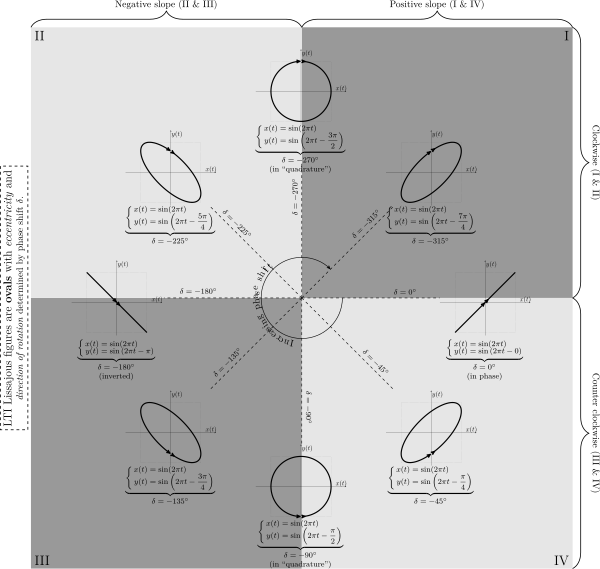
\includegraphics[width=0.9\textwidth]{Lissajous.png}
    \caption{Lissajous figures}
    \label{fig:Lissajous-png}
\end{figure}

\end{document}
